\documentclass[10pt,a4paper]{beamer}

\usepackage[utf8]{inputenc}
\usepackage[russian]{babel}
\usepackage[OT1]{fontenc}
\usepackage{amsmath}
\usepackage{amsfonts}
\usepackage{amssymb}
\usepackage{makeidx}
\usepackage{graphicx}
\usepackage{xcolor}
\usepackage{multirow}
\usepackage{framed}
\definecolor{shadecolor}{cmyk}{0,0,0,1}
\usepackage{hyperref}
\usepackage[normalem]{ulem}
\usepackage{wasysym}

\titlegraphic{
   
\includegraphics[width=4cm]{images/sfera.jpg}
}

\author{Николай Анохин \and Михаил Фирулик}
\title{Введение в Data Science \\ Занятие 10. Метод ансамблей}

\beamertemplatenavigationsymbolsempty

\begin{document}

\maketitle

\logo{
    
\includegraphics[width=4cm,keepaspectratio]{images/sfera.jpg}\hspace{0.45em}
}

\begin{frame}

\tableofcontents

\end{frame}

% ============================================== %

\section{Метод ансамблей}

% ============================================== %

\begin{frame}{Задача классификации}

Пусть дана выборка, состоящая из обучающих объектов 
\[
\mathbf{X} = (\mathbf{x}_1, \ldots, \mathbf{x}_N),
\]  
и соответствующих значений целевой переменной 
\[
Y = (y_1, \ldots, y_N) = (f(\mathbf{x}_1), \ldots, f(\mathbf{x}_N)).
\]
Требуется найти функцию $h(\mathbf{x})$, наилучшим образом приближающую $f(\mathbf{x})$, то есть точно предсказывающую значение целевой переменной для любых $\mathbf{x}$.

\end{frame}

% ============================================== %

\begin{frame}{Недостатки одиночных моделей}

\begin{itemize}
\item Statistical issue \\
{\it риск выбрать неправильную гипотезу из возможного набора, учитывая ограниченность выборки}
\item Computational issue \\
{\it риск получить локальный минимум в результате оптимизации}
\item Representational issue \\
{\it риск, что ни одна из моделей не окажется достаточно хорошей}
\end{itemize}

\end{frame}

% ============================================== %

\begin{frame}{Метод ансамблей}

\begin{center}
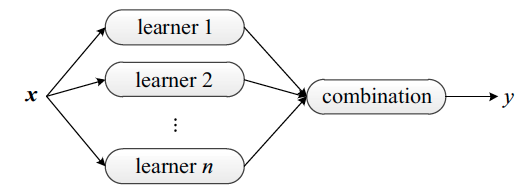
\includegraphics[scale=0.5]{images/ensemble.png}
\end{center}

\begin{block}{Идея}
Построить несколько {\bf базовых моделей} и правильным образом {\bf скомбинировать} их для принятия решения. В идеале базовые модели должны быть максимально {\it точными} и при этом {\it разнообразными}.
\end{block}

\end{frame}

% ============================================== %

\begin{frame}{Виды ансамблей}

\begin{itemize}
\item комбинация классификаторов (combining classifiers) \\
{\it pattern recognition}
\item ансамбль слабых моделей (ensemble of weak learners) \\
{\it machine learning}
\item смесь экспертов (mixture of experts) \\
{\it neural networks}
\end{itemize}

\end{frame}

% ============================================== %

\begin{frame}{Стоит ли?}



\begin{columns}[C]
    \begin{column}{.5\textwidth} 
	\begin{itemize}
	\item Рекомендательные системы \\ 
	{\it Победитель Netflx Prize \$1M (первое и второе места)}
	\item Компьютерное зрение \\ 
	{\it AdaBoost with cascade -- определение лиц на фото (или стыковка с МКС \blacksmiley{})}
	\item Медицинская диагностика \\
	{\it Определение болезни на ранней стадии}
	\end{itemize}    
    \end{column}
    \begin{column}{.5\textwidth} 
    \vspace{0em}
    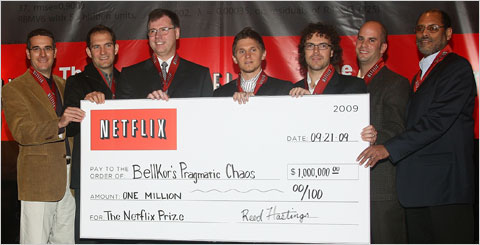
\includegraphics[scale=0.33]{images/netflix.jpg}    
    \end{column}
\end{columns}

\end{frame}

% ============================================== %

\section{Boosting}

% ============================================== %

\begin{frame}{Boosting}

Пусть дан алгоритм обучения ``слабой'' модели -- такой, которая только немного 				лучше случайности
\vspace{1em}

\begin{columns}[C]
    \begin{column}{.5\textwidth} 
	\begin{block}{Идея метода}	
		Последовательно обучать слабые модели так, что каждая следующая модель 						``исправляет ошибки'' предыдущих. Для предсказания используется комбинация из 			всех моделей последовательности.
	\end{block}		    
    \end{column}
    \begin{column}{.5\textwidth} 
    \vspace{-1em}
    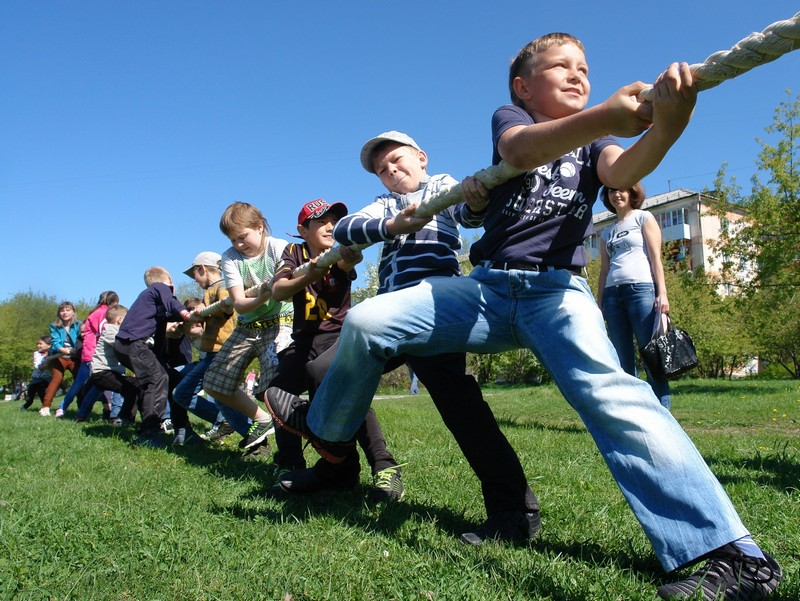
\includegraphics[scale=0.18]{images/children.jpg}    
    \end{column}
\end{columns}

\end{frame}

% ============================================== %

\begin{frame}{AdaBoost}

\texttt{ada\_boost($\mathbf{X}$, $Y$, $T$):}

\texttt{\quad инициализируем $\mathcal{D}_1 = 1/m$}

\texttt{\quad for $t = 1, \ldots, T$:}

\texttt{\quad\quad обучаем модель $h_t(\mathbf{x}) = \mathcal{L}(\mathbf{X}, Y)$,}

\texttt{\quad\quad\; принимая во внимание распределение $\mathcal{D}_t$}

\texttt{\quad\quad вычисляем ошибку $h_t(\mathbf{x})$: $\epsilon_t = P_{\mathbf{x} \sim \mathcal{D}_t}(h_t(\mathbf{x}) \neq f(\mathbf{x}))$}

\texttt{\quad\quad if $\epsilon_t > error\_rdm$:} 

\texttt{\quad\quad\quad break}

\texttt{\quad\quad вычисляем  вес $h_t(\mathbf{x})$: $a_t = \frac 1 2 \ln(\frac{1-\epsilon_t}{\epsilon_t})$}

\texttt{\quad\quad новое распределение: $\mathcal{D}_{t+1}(\mathbf{x}) = \frac{\mathcal{D}_t(\mathbf{x})}{Z_t} \exp(- a_t f(\mathbf{x}) h_t(\mathbf{x})) $}

\texttt{\quad return $H(\mathbf{x}) = \text{sign} \sum_{t=1}^T a_t h_t(\mathbf{x})$}

\end{frame}

% ============================================== %

\begin{frame}{Свойства AdaBoost}

\begin{itemize}
\item Минимизирует экспоненциальную ошибку (exponential loss)
\[
L_{exp}(h | \mathcal{D}) = E_{\mathbf{x} \sim \mathcal{D}} [e^{-f(\mathbf{x})h(\mathbf{x})}]
\]
\item Требует обучения модели с учетом распределения \\
{\it Варианты: re-weighting или re-sampling}
\item Ошибка классификации
\[
\epsilon_\mathcal{D} \leq \epsilon_{\mathbf{X}} + O \left(\sqrt{\frac{dT}{N}}\right)
\]
($d$ отражает ``сложность'' классификатора)
\end{itemize}

\end{frame}

% ============================================== %

\begin{frame}{AdaBoost: тесты}

\begin{center}
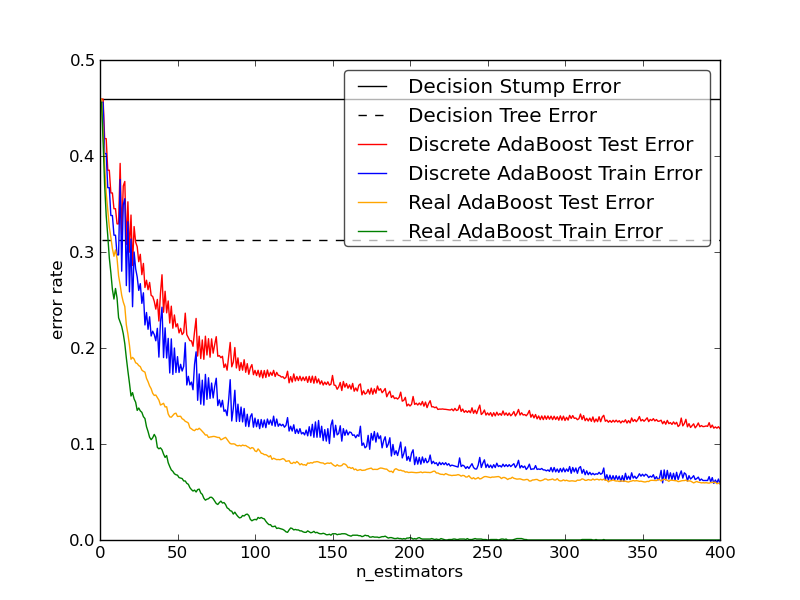
\includegraphics[scale=0.25]{images/ada.png}\;
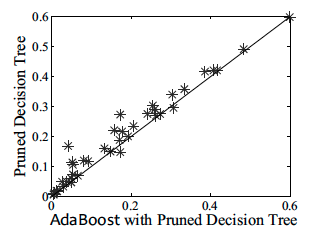
\includegraphics[scale=0.42]{images/ada2.png}

\hspace{17em}
\includegraphics[scale=0.2]{images/uci.png}
\end{center}

\end{frame}

% ============================================== %

\begin{frame}{Пример}

\vspace{-2em}
\begin{center}
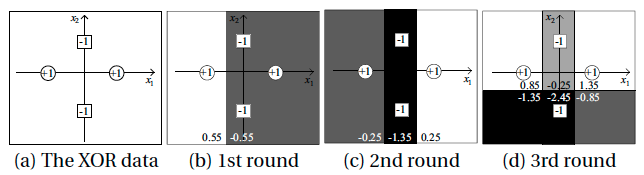
\includegraphics[scale=0.5]{images/xor.png}
\end{center}

\vspace{-2em}
\begin{small}
\[
h_1(\mathbf{x}) = \begin{cases}
+1, \text{ если } x_1 > -0.5 \\ 
-1, \text{ иначе }
\end{cases} \quad
h_2(\mathbf{x}) = \begin{cases}
-1, \text{ если } x_1 > -0.5 \\ 
+1, \text{ иначе }
\end{cases}
\]
\[
h_3(\mathbf{x}) = \begin{cases}
+1, \text{ если } x_1 > +0.5 \\ 
-1, \text{ иначе }
\end{cases} \quad
h_4(\mathbf{x}) = \begin{cases}
-1, \text{ если } x_1 > +0.5 \\ 
+1, \text{ иначе }
\end{cases}
\]
\[
h_5(\mathbf{x}) = \begin{cases}
+1, \text{ если } x_2 > -0.5 \\ 
-1, \text{ иначе }
\end{cases} \quad
h_6(\mathbf{x}) = \begin{cases}
-1, \text{ если } x_2 > -0.5 \\ 
+1, \text{ иначе }
\end{cases}
\]
\[
h_7(\mathbf{x}) = \begin{cases}
+1, \text{ если } x_2 > +0.5 \\ 
-1, \text{ иначе }
\end{cases} \quad
h_8(\mathbf{x}) = \begin{cases}
-1, \text{ если } x_2 > +0.5 \\ 
+1, \text{ иначе }
\end{cases}
\]
\end{small}

\end{frame}

% ============================================== %

\begin{frame}{Еще boosting}

\begin{itemize}
\item LogitBoost
\[
L_{log} (h | \mathcal{D}) = E_{\mathbf{x} \sim \mathcal{D}} \left[ \ln \left(1 + e^{-2 f(\mathbf{x}) h(\mathbf{x})}\right) \right]
\]
\item GradientBoosting \\
{\it оптимизация произвольной функции потерь + регуляризация}
\end{itemize}

\begin{center}
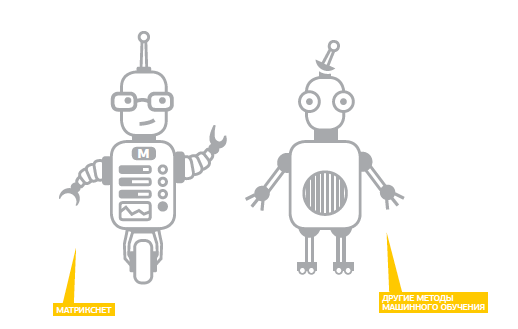
\includegraphics[scale=0.35]{images/matrixnet.png}
\end{center}

\end{frame}

% ============================================== %

\begin{frame}{AdaBoost. Итоги}

\begin{itemize}
\item[+] Высокая точность
\item[+] Почти не переобучается
\item[---] Трудно параллелизовать
\item[---] Чувствителен к шуму
\end{itemize}

\end{frame}

% ============================================== %

\section{Bagging}

% ============================================== %

\begin{frame}{Bagging}

Bagging = Bootstrap + Aggregating

\vspace{1em}

\begin{block}{Идея метода}
Обучить несколько независимых моделей на основании случайно выбранных (bootstrap) подмножеств объектов из обучающей выборки. Классификация производится на основании результата голосования (aggregating) моделей.
\end{block}

\end{frame}

% ============================================== %

\begin{frame}{Bagging}

\texttt{bagging($\mathbf{X}$, $Y$, $T$):}

\texttt{\quad for $t = 1, \ldots, T$:}

\texttt{\quad\quad генерируем bootstrap-распределение $\mathcal{D}_{bs}$}

\texttt{\quad\quad обучаем модель $h_t(\mathbf{x}) = \mathcal{L}(\mathbf{X}, Y)$,}

\texttt{\quad\quad\; принимая во внимание распределение $\mathcal{D}_{bs}$}

\texttt{\quad return $H(\mathbf{x}) = \arg \max_{y \in Y} \sum_{t=1}^T \mathbf{I}(h_t(\mathbf{x}) = y)$}

\end{frame}

% ============================================== %

\begin{frame}{Bagging: тесты}

\begin{center}
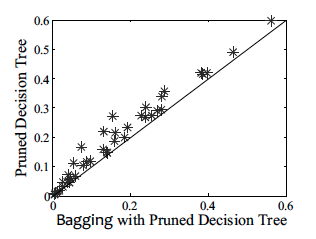
\includegraphics[scale=0.4]{images/bag1.png}\;
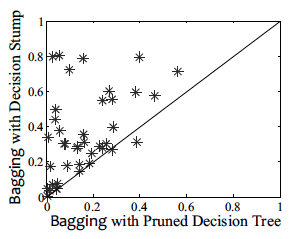
\includegraphics[scale=0.4]{images/bag2.png}
\end{center}

\end{frame}

% ============================================== %

\begin{frame}{Random Forest}

\texttt{random\_tree($\mathbf{X}$, $Y$, $K$):}

\texttt{\quad $N$ -- узел дерева для $\mathbf{X}$}

\texttt{\quad if все $\mathbf{x} \in \mathbf{X}$ одного класса:}

\texttt{\quad\quad return $N$}

\texttt{\quad $\mathcal{F}$ -- случайно выбираем $K$ признаков}

\texttt{\quad $f \in \mathcal{F}$ -- признак, наилучшим образом разделяющий $\mathbf{X}$}

\texttt{\quad $N_l = random\_tree(X_l^f, Y_l^f, K)$ }

\texttt{\quad $N_r = random\_tree(X_r^f, Y_r^f, K)$ }

\texttt{\quad добавляем $N_l$ и $N_r$ как детей к $N$}

\texttt{\quad return $N$}

\end{frame}

% ============================================== %

\begin{frame}{Random Forest: тесты}

\begin{center}
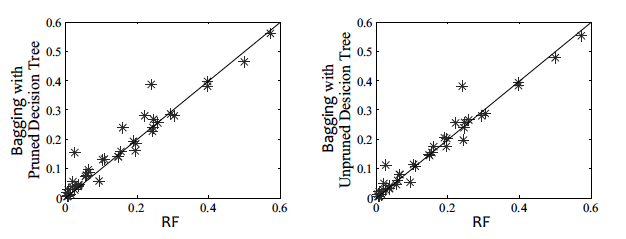
\includegraphics[scale=0.5]{images/rf.png}
\end{center}

\end{frame}

% ============================================== %

\begin{frame}{Модификации Random Forest}

\begin{itemize}
\item VR-Tree \\
{\it В каждом узле с вероятностью $\alpha$ просиходит случайный выбор признака}
\item Density estimation \\
{\it Польностью случайное дерево}
\item Anomaly Detection \\
{\it Польностью случайное дерево с ограничением по глубине SCiForest}
\end{itemize}

\end{frame}

% ============================================== %

\begin{frame}{Density Estimation}

\begin{center}
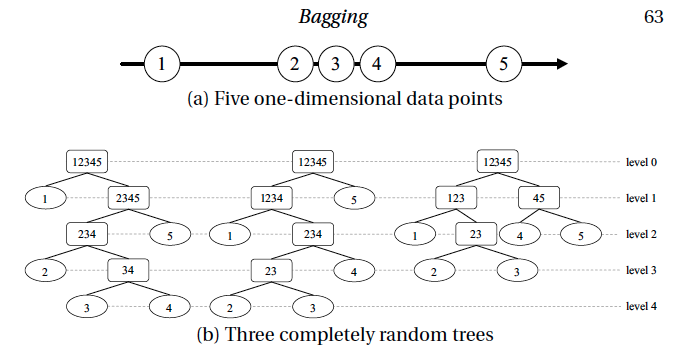
\includegraphics[scale=0.25]{images/de1.png}
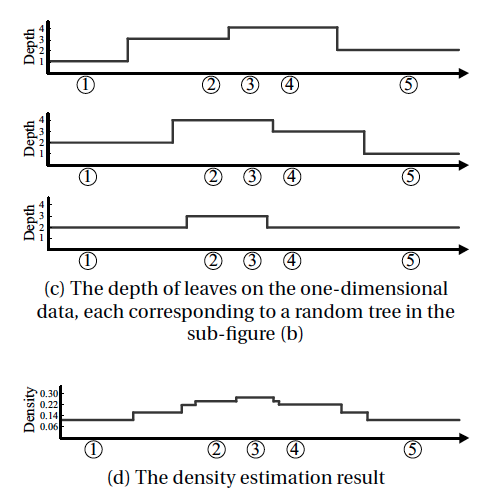
\includegraphics[scale=0.25]{images/de2.png}
\end{center}

\end{frame}

% ============================================== %

\begin{frame}{Random Forest. Итоги}

\begin{itemize}
\item[+] Высокая точность
\item[+] Мало переобучения
\item[+] Легко параллелится
\item[---] Медленный без параллелизма
\end{itemize}

\end{frame}

% ============================================== %

\begin{frame}{Сравнение методов}

\begin{center}
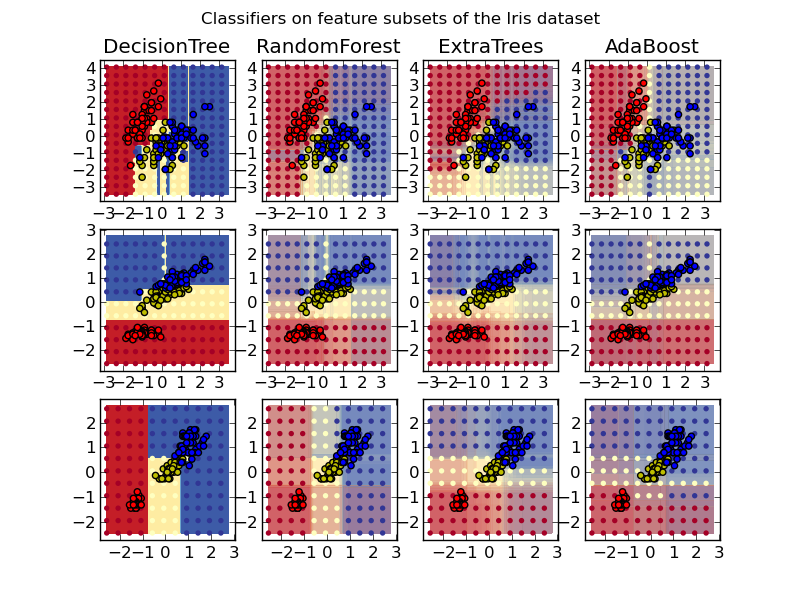
\includegraphics[scale=0.45]{images/comp.png}
\end{center}

\end{frame}

% ============================================== %

\section{Комбинирование моделей}

% ============================================== %

\begin{frame}{Зоопарк комбинаций}

Задача регрессии
\begin{itemize}
\item averaging
\item weighted averaging
\end{itemize}

Задача классификации
\begin{itemize}
\item majority voting
\item plurality voting
\item weighted voting
\item soft voting
\end{itemize}

Кроме того: stacking

\end{frame}

% ============================================== %

\begin{frame}{Выводы}

\begin{center}

\includegraphics[scale=0.65]{images/forest.jpg}
\end{center}

\end{frame}

% ============================================== %

\begin{frame}[fragile]{Задача. Распознавание цифр}

Дана обучающая выборка с картинками 8x8, на каждой из картинок изображена рукописная цифра.

\begin{shaded}
{\color{green} \begin{verbatim}
$ python digits.py -s 25
\end{verbatim}}
\end{shaded}

\begin{enumerate}
\item для алгоритма AdaBoost построить график зависимости $train\_error$ и $test\_error$ от $T$
\item для алгоритма RandomForest построить график зависимости $train\_error$ и $test\_error$ от размера леса
\item реализовать простейший голосующий ансамбль и исследовать зависимость его точности от вида и количества базовых моделей
\end{enumerate}

\end{frame}

% ============================================== %

\end{document}